\chapter{Discussion and Future Work}
\label{Discussion}

\section{Introduction}
\label{Discussion:Intro}
In the remainder of this chapter, I revisit the main research aim :
\begin{quote}
\textbf{\textit{``How might participation be configured for people with dementia to shape the design process of technology''}}
\end{quote}

The subsection below explores the lessons learned across the data chapters and is split into the three research questions I set out at the start of the thesis. After reviewing the research questions, I reimagine the role of participation between people with dementia and diverse stakeholders to move towards a more inclusive design space that supports mutuality in the co-creation of new technologies and systems. 

\section{Participatory approaches}
\label{Discussion:RQ1}
\begin{quote}
\textbf{    Research Question 1:
}    
\textit{    “How can we use participatory design approaches to provide meaningful and engaging experiences for people with dementia?”}
\end{quote}


\section{Ethical implications in dementia and HCI}
\label{Discussion:RQ2}
\begin{quote}
\textbf{    Research Question 2:
}    
\textit{    “What are the ethical implications for people with dementia to participate in HCI research?”}
\end{quote}

Across the studies in this thesis, I have examined various ethical challenges underpinning research in the area of dementia. As seen in chapter six, significant attention to these ethical dilemmas is emerging in dementia-HCI researchers' works. A significant part of these conversations looks toward strategies and frustrations involving people with dementia in ethical and inclusive ways. In many of the examples in this thesis, multiple ethical challenges in involving people with dementia stemmed from attaining consent and researching under a culture of ethical 'protectionism'. To answer the research question, I have split this section into the following: a) implications for attaining consent; b)  building community understanding for ERBs; and c) involving those further under-represented in dementia.

\subsection{Implications for consent}
\label{Cosent-Implications}
In chapter six, many of the researchers stressed the tendency for ethical review boards (ERBs) to see people with dementia as 'vulnerable'. \cite{pachana_can_2014} further highlights that committees may be \textit{``subject to the same biases and stereotypes present in the general population''}. ERBs that are unaware of such biases, may focus on the aims of protection, as opposed to the approval of research that attends to topics such as agency and ensure meaningful participation. For instance, as I describe in chapter four, Philip could not provide informed consent to participate at the given moment. In accordance to the Mental Capacity Act (2005) that the university follows:

\begin{quote}
\textit{``A person lacks capacity in relation to a matter if at the material time he is unable to make a decision for himself in relation to the matter because of an impairment of, or a disturbance in the functioning of, the mind or brain.''} \citep{oyebode_mental_2005}
\end{quote}

As demonstrated in chapter four, Philip's ability to make decisions seems to fluctuate depending on the time of day, and interactions throughout the day. However, that might suggest that the consent procedure should be taken when the person with dementia is having a 'better day' than other days, which still restricts a very ambiguous process and requires flexibility \citep{trachsel2015cognitive}. 

\cite{o2021advocating} argue that \textit{``although a person with dementia may have been deemed to lack capacity to make complex life decisions, it does not necessarily follow that they will not have capacity' to understand the general nature and activities of a study''}. \cite{dewing_participatory_2007} describes a process of consent that centres on the individual's values and interests. Through this process, Dewing suggests that those who cannot legally formally consent can still engage through 'inclusionary consent' based on experiential preferences that come from building researcher-participant relationships. Further, Dewing stresses that the consent process should continue through the research process.

\subsection{Connecting ERBs with community members}
\label{ERBs-Community-Members}
In chapter six, researchers raised a range of concerns with ERBs when the ERB does not have the specialisation on the topic at hand. As several researchers report, this may result in the committee orienting towards a biomedical view of dementia causing several knock-on effects of getting ethics approved. One option would be for researchers to provide training support to committee members on the topics of dementia. For instance, \cite{goldberg2015relationship} reviews a dementia-focused Massive Open Online Course (MOOC), demonstrating a significant reduction in stereotypical assumptions on the capabilities of people with dementia. However, adopting such an approach would require committee members to take courses and training for other non-expert topics, which would not be possible given how many topics ERBs have to consider. 

Alternatively, \cite{lidz2012participation} reports on community members' participation on a medical institutional review board. While the authors describe issues regarding community members playing a lesser role than other institutional members, the authors convey value to community members by providing helpful insight into consent processes and essential topics of confidentiality and privacy. Similarly, in the thesis, I have described several times where researchers should consider ways to build conversational tools for community members and ERBs that promotes conversation and inclusion. \cite{davies2021dementia} co-authored a paper with six people with dementia that explores Dementia Enquirers, a dementia advocacy group, who are developing ethical guides and best approaches for dementia research to support the design and development of ethical designed dementia research. For researchers, next steps might want to consider how we might connect advocacy groups (like Dementia Enquirers), to the unviersity ERB committees. With Dementia Enquirers building an ethics panel and their DEEP-Ethics Gold Standards, perhaps institutional ethics might consider inviting these community-led panels to handle ethical issues and approvals on behalf of the community they represent. That way, people with dementia can provide valuable pre-design feedback and ensure research designs are rooted in community-led agendas. 


\subsection{Involving people further under-represented in dementia.}
\label{Under-represented--dementia}
Within HCI, there is increased attention to incorporating the voices of underrepresented populations to support issues of health, wellbeing and political engagement \citep{erete_intersectional_2018}. \cite{harrington_forgotten_2020} describes that HCI research is beginning to see researchers acknowledging that they are groups or communities who sit at the 'forgotten margins'. These margins comprise of marginalised people with multiple identities, who are continued to be neglected by research and design efforts. For instance, these groups are people who might identify as people with dementia, but have cultural or sexual identities that further marginalise that person or group. 

From the work I conducted in the North East, the families I worked with were predominantly from a working-class background, white and in a heterosexual relationship. Given that only 11\% of Newcastle's total population are black, asian or minority ethnic (BAME), it is no surprise that the members of Silverline Memories came from very similar upbringings and backgrounds \citep{cityCouncil_2021}. Meanwhile, in chapter seven, I worked with a number of people with dementia from mixed backgrounds, such as an accountant, human rights lawyer, and social worker. In particular, Masood originally came from Pakistan and moved to the UK as a teenager. When interviewing Masood, I became aware of several implications that might make participation challenges that had not become apparent in my prior work. For instance, Masood mentioned how much of the diagnosis content he received was in English. However, he stresses that \textit{`` for others whose English is their second language, accessing these useful resources is extremely inaccessible''} \citep{cooper2018relationship}. Masood continued by emphasising that linguistic and cultural barriers would contribute to his family \textit{``having a lack of understanding about dementia, who would sometimes have offensive views of dementia''}. In. this way, from the interviews with Masood, I gained unique understandings that are not apparent in conversations with people at Silverline Memories . 

With this in mind, researchers might want to consider how we might invite and involve groups that are further underrepresented, such as, the LGBTQ+ community, young onset dementia, advanced dementia and people with other cultural and diverse backgrounds \citep{foley_struggle_2019, bryden_before_2015} (McGovern, 2014). \cite{mcgovern2014forgotten} describes designing spaces for safety and belonging that provide people with dementia in the LGBTQ community to open up and share their stories. The authors suggest that to build a meaningful and safe space, researchers should accept diversity; adopt language that represents the community; and use language and images that represent the LGBTQ community during recruitment, whether in information sheets, marketing materials, or leaflets. Further, when talking with Howard who is a dementia advocate for 3 Nations Working Group, he mentioned that the group has \textit{``started to get people from ethnic, LGBTQ+ backgrounds, but it is still far from being done...''}. As researchers often have the unique opportunity of working with those who are under-represented, researchers should consider that part of their research impact is to build connections between participants and dementia networks to support the growth and inclusivity of networks that are making change. 

\subsection{Summary}
\label{EthicsSummary}
From this section, the main point here is that there are several barriers to dementia that stop research and practice from being more inclusive and meaningful. However, to move towards a practice that ensures people with dementia are valued and can participate and contribute to the extent they want to, we might consider the following:
\begin{itemize}
    \item Educate members of ERBs, and others, about the ramifications that a biomedical view portrays.
    \item Manage relational dynamics (between family members and the person with dementia).
    \item Researchers to create connections between participants from underrepresented communities in other dementia networks.
    \item Tailor the consent process to the needs and requirements of the person with dementia.
\end{itemize}

\section{Supporting meaningful dialogue}
\label{Discussion:RQ3}
\begin{quote}
\textbf{    Research Question 3:
}    
\textit{ “What are the competing interests and expectations to support meaningful dialogue in dementia design research when involving multiple stakeholders - such as people with dementia, developers, designers and researchers?”}
\end{quote}

\subsection{Stakeholders implicated in the design process}
\label{DevsDesigners}
At a time when technology has become increasingly complex, adopted into our daily lives, and ubiquitous, researchers are drawing attention to the design and deployment of technology. For instance, in recent years, HCI researchers have begun recognising the 
real-world harms that AI integrations may cause. In response, the AI community has worked closely with activists and advocacy groups to find ways to learn and support their work to empower communities through tools or systems for understanding data collection. One popular approach in teaching methods on accountability and transparency has been through the building of toolkits. For instance, Katell et al. co-designed an Algorithmic Equity Toolkit that provides AI researchers reflective questions to surface the social context of the system, and activities to better understand how machine learning works and how it fails. The processes to improve the ethical design of AI resonates with Mulvenna et al. manifesto called 'Ethical by Design'. The manifesto proposes several principles such as 'seek to integrate with and support the progression of policy'; 'Be realistic about what is possible and needed; "provide enough information for people to make informed decisions at every stage about whether, when and, and how to use the product or service'. 

In chapter seven, three of the four developers expressed that while they "know [their] designs should be more considerate and ethical,   but when they are time constraints and a limited team, there is only so much [they] can do". In this way, designing approaches to provide more ethical solutions in technology design requires considering how toolkits and approaches fit into the designer's or developer's workflow. However, fitting into workflows seemed insufficient to ensure meaningful collaboration between stakeholders and people with dementia. In chapter five, the hackathon demonstrated that while prize money was a contributor to participating in the weekend, multiple teams indicated pro-social motivations where teams like Garden Life, were driven to ``deepen [their] understanding of these issues'' in the hope of ``alleviating the stigma''. Similarly, when talking about community-led projects in chapter seven, Husainah suggested how some designers may contribute because their skillset could help others. However, Husainah and other designers did say they would only contribute in small amounts where they might provide help on a weekend or evenings. 

In summary, through the thesis, designers and developers have shown a keen interest in working with people with dementia, mainly where it provides learning opportunities or the chance to help others. However, at the same time, designers and developers expressed that supporting that dialogue in the development of technology can become challenging when it collides with their workflows, even when they explicitly acknowledge the importance of involving the voices of the users they are designing for. Chapter seven highlights these complications further where participants described such reflective work with people with dementia can be tricky in private sector areas where more user-focused projects require longer-term projects with potentially larger budgets.

\subsection{People with dementia and care partners}
\label{PwDInterests}
Across the thesis, people with dementia expressed several expectations when participating and contributing to design work, ultimately providing a more supportive space for conversation between people with dementia and stakeholders. Within dementia advocacy, a recent movement mirrors the disability rights and disability justice activists who popularised the phrase ``nothing about us without us''. For example, Dementia Alliance International uses this term in their stated goal of eradicating stigma and discrimination and recognises the eligibility for anti-discriminatory disability rights for both people with dementia and their supporters. Through this, we have seen a rise in advocacy groups and advocates campaigning for change through blogs, keynotes, and other campaigning activities to discuss the social and individual challenges of living with dementia (Thoma and Milligan).

In chapter seven, I worked closely with people with dementia who are advocates for building a collaborative toolkit to support the design for dementia. During the interviews, people with dementia raised concerns about the lack of recognition they get when participating in the design process. In one instance, Masood described frustrations of ``feel[ing] like a guinea pigs'' where once the designers have the information they need, they would leave and not acknowledge Masood for his contribution. Similarly, the participants said they are often 'giving' away their experiences and expert knowledge for free. Despite being invited into a design process with paid designers and developers, there is little expectation from corporate companies to pay these advocates for their time.

Similarly, Bartlett et al. interviewed campaigners living with dementia who reported a psycho-emotional burden through campaigning where people would comment on how the campaigner contradicts dementia 'norm' to the extent they felt like a fraud. In this way, through the thesis, people with dementia have expressed explicit interest and want to be part of the participatory process and design alongside other stakeholders. However, when treated as unequal and not recognised for their contribution, participants described disinterest and exhaustion of their continued work as advocates. 







\section{Meaningful participation in design approach}
\label{Discussion:Design}

\begin{figure}[htp]
\centering
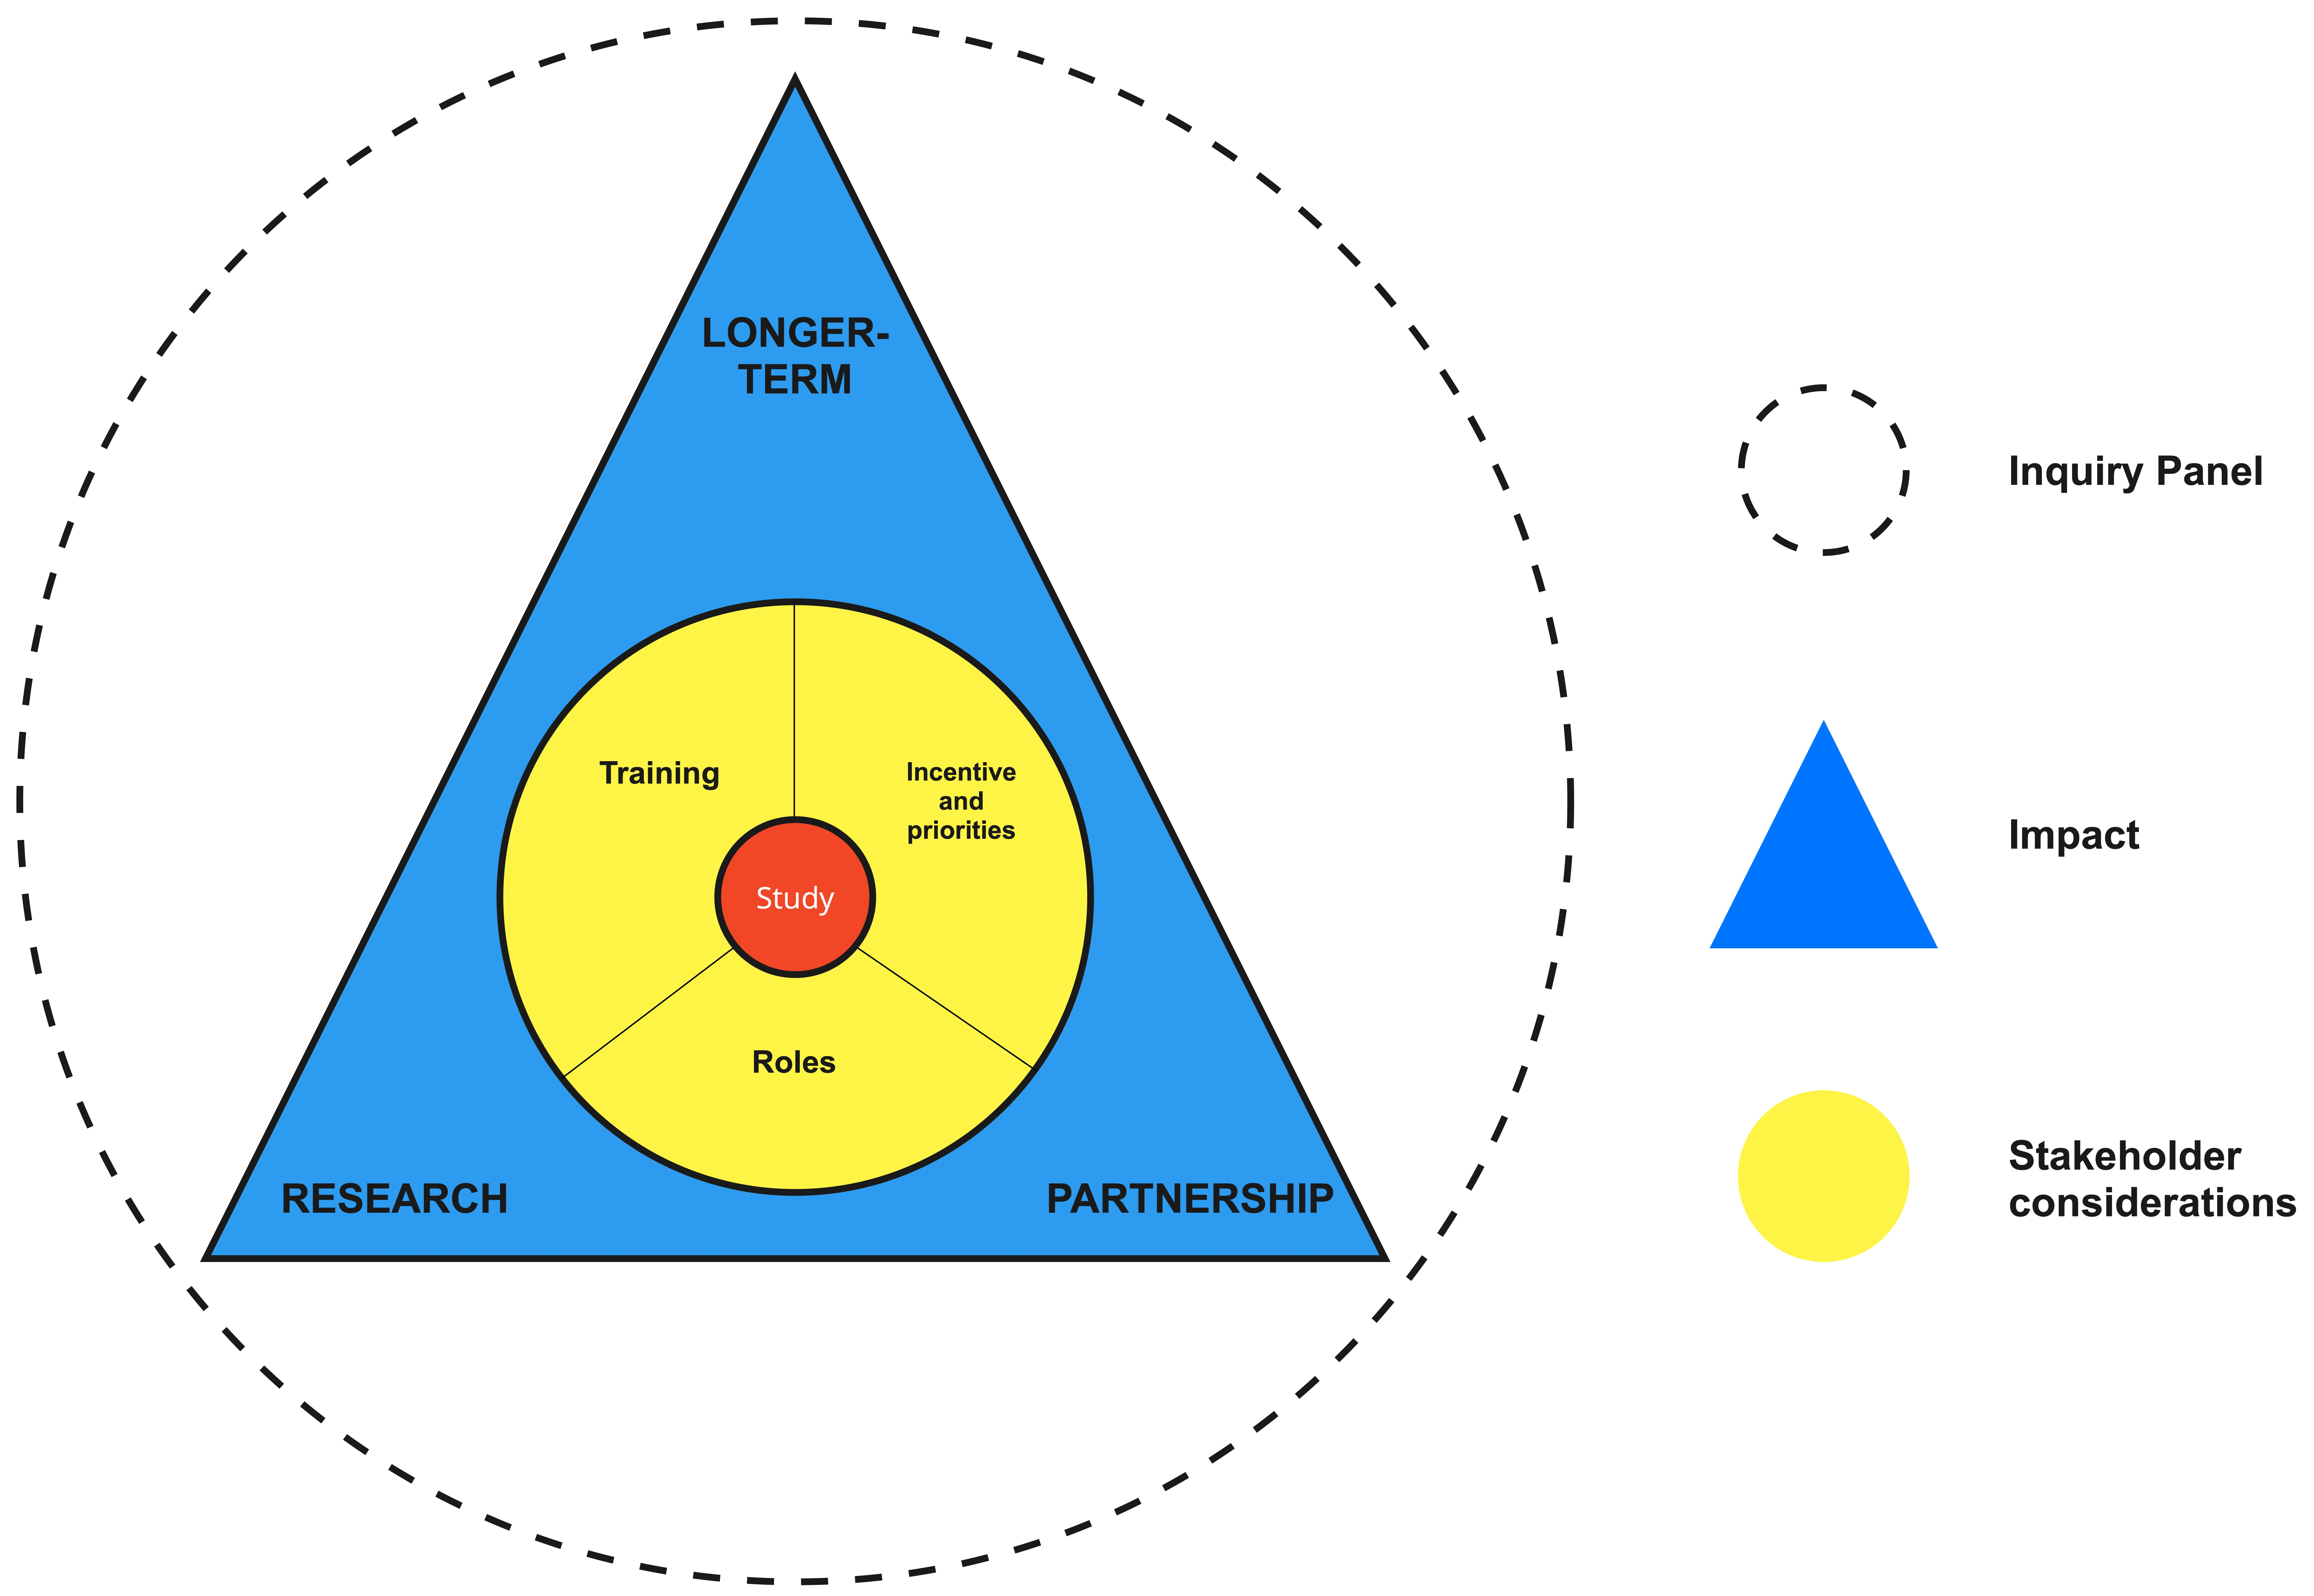
\includegraphics[width=0.8\linewidth]{Images/Discussion/DesignApproach.jpg}
\caption{Meaningful participation in design diagram}
\label{fig:MeaningfulParticipation}
\end{figure}
The meaningful participation design approach draws on the insights from the previous data chapters to meaningfully engage and broaden the dementia debate through a more inclusive approach. The approach consists of three core components that surround a research study. By considering the three components, the aim is for researchers to critically reflect and consider ways to improve stakeholder engagement, ethically engage with research impact, and ensure research designs are rooted in participant-led agendas. The three components are the following:

\begin{itemize}
    \item \textbf{Inquiry Panel}: Developing a group of experts (primarily stakeholders) who guide and shape the research and provide answers to any queries by the research team.
    \item \textbf{Impact}: Consists of three critical areas that researchers should consider when designing engaging and impactful outputs for their studies.
    \item \textbf{Stakeholder considerations}: A set of three considerations to move towards more inclusive and engaging research that articulates the interests and priorities of the stakeholders the research will impact.
\end{itemize}

\subsection{Inquiry panel}
\label{Inquiry Panel}
As described throughout the PhD, a key concern I raise is participants' lack of influence on research agendas. Similarly, \cite{suijkerbuijk_active_2019} highlight that people with dementia are often underrepresented in pre-design and generative phases of technology development. By ensuring research designs are rooted in participant-led agendas, they can contribute to a more ethical, engaged research study. As \cite{dupuis_moving_2012} argue, \textit{"listening and hearing the perspectives of persons with dementia is not enough. We must actively involve them in decision-making to the fullest of their abilities and support their involvement using whatever means necessary" (p.433)}. One common approach that has gained recent attraction in the last few years is the development of dementia activist groups which aim to promote the voices of people with dementia and guide and shape the design of research approaches \citep{weetch2021involvement}. Working with activist groups contextualises a deeper understanding of what work is sensitive and what is not. It also articulates the interests and priorities of the individuals the research will impact. As such, part of the meaningful participation design approach builds upon these activist groups by suggesting that researchers might implement an Inquiry panel in their research.

The Inquiry panel consists of people who have expertise in the domain the research is looking into. For instance, this thesis inquiry panel would involve people with dementia, care partners, developers, designers, and researchers. From here, the research team actively involves the inquiry panel in designing research agendas, feedback on ethical and methodological approaches, and supporting recruitment. By building a panel of experts to support the research team's ideas and approaches, the panel echoes prior work that supports confidence building, empowerment, and providing opportunities for change and development.

Furthermore, a more diverse group of experts within the inquiry panel might enable the building of reciprocal relationships with other members by learning and sharing their expertise and experiences. However, it is worth noting that building a diverse set of voices and backgrounds will require careful consideration and facilitation to ensure voices are represented. For instance, \cite{innes2021s}, who worked with The Dementia Associate Panel (DAP), a group of people with dementia who advocate for change and policymaking, described the panel's ongoing flexibility and adaption to facilitation to ensure meaningful participation. The author used \textit{"self-reported questionnaires at the end of each [panel] meeting...which allowed [the members] to indicate whether the meeting effectively supported their contribution of view and ideas"}. While this thesis describes the need for broadening stakeholders to be involved in the entire research process, it will need the creation of tools and approaches to promote conversation and inclusion of community members, researchers, and other infrastructures that uphold our work i.e., ethical review boards and grant panels. 

To conclude this section, I suggest a set of steps that may be useful for researchers who want to start and develop an inquiry panel:

\begin{itemize}
    \item List the potential groups/people that have expertise on a specific topic (people with dementia, family members, researchers).
    \item Invite these experts to take part in the panel. You may find these people through other advocacy/network groups.
    \item To facilitate inclusive meetings, ask the panel members a) if they understand the project/panel and b) if they require any additional support or practicalities to make their involvement easier, e.g., invitation, signage, refreshments if in person.
    \item At the first meeting, as the researcher, prepare a presentation that describes your plans for the potential project, how long it will be, and the potential outputs/expectations. Following, open the conversation up to the panel to discuss the issues and interests of the project.
    \item As the research team, you might want to write summary emails and design an ongoing report that disseminates the conversations from the meetings. 
    \item To maintain interest from the panel, you should continue to engage with them monthly to provide updates and ask for any necessary feedback. For instance, if you stumble on ethical challenges with your ERB, you might want to ask dementia experts about the best ways to promote ongoing consent. 

\end{itemize}

\subsection{Impact}
\label{Impact}
In the following section, I unpack three key areas that researchers should consider to provide insight into the study's potential value for research, the community, and the longer-term impact.

\subsubsection{Research impact}
When considering research impact, there is a distinction between the intellectual contribution to the field and the area beyond academia. For within the field, publications and workshops are a well-established way to contribute to the knowledge of the domain. For instance, the work in chapter six was published in 2020 to disseminate the ethical challenges dementia-HCI researchers might face when working in everyday settings. In this example, the paper and presentation video were targeted at a niche but relevant group of people who might read an academic publication. A month later after the paper and video were published and shared across Twitter, I received this email:


\begin{quote}
\textit{My name is Jim Mann, I reside in Canada’s western most province, British Columbia and I have Alzheimer's. I am an active community member as an advocate, a committee member and a co-investigator, collaborator in various research projects.} 

\textit{Ethics in research with people with dementia and the actions of Research Ethics Boards have been a concern of mine for a number of years. In 2018 I spoke at the Canadian Association of Research Ethics Boards annual meeting and, at the invitation of the University of British Columbia’s W. Maurice Young Centre for Applied Ethics, I was invited to be a Visiting Community-Based Scholar in July 2019 where I focused on dementia research and issues of consent and ethics. And last year I was invited to join the Advisory Council of Research Ethics BC alongside ethics professionals. I provide this information to illustrate my continued concern in this area.
} 

\textit{Including mention of anonymous contributions made me smile because it was only a few years ago that I alongside Dr. Deb O’Connor and Dr. Elaine Wiersma had an article accepted for publication. My affiliation was listed as ‘Dementia Advocate,’ which became a sticking point because that was not considered a ‘real’ affiliation. Eventually it was accepted but it showed all of us how the contribution of a ‘patient’, a person with dementia was not deemed relevant. In my presentation, the link to which I’ve included, I speak of a “researcher’s ethics application that included the point that participants names would be published with their consent. In the words of that researcher, the idea seemed outrageous to the ethics board and after seven months she was still awaiting approval.
} 

\textit{So, I send you and your team my best wishes as you move forward in your studies and careers.
}
\end{quote}

Jim, who later became a participant in the chapter seven study, sent this email with the kindest regards to myself and the other collaborators. In this example, the academic publication had reached someone with dementia. However, Jim has extensive insight into the research domain and continues to work with well-known dementia researchers such as \cite{bartlett2010broadening}. While research outputs help provide new insights and lessons for the academic community, publications are usually not read outside the academic space. As suggested in Chapter six - DemVR, researchers might want to consider disseminating their research into less 'static' ways to offer insights and novel methodological approaches to a broader audience. \cite{smith2020disseminating} recent qualitative study describes ways to mitigate potential barriers to dissemination of research to the public. For instance, the authors suggest researchers might consider removing topic jargon, reading comprehension levels, and exploring accessible narratives to mitigate miscommunication in their research. Therefore, to get the public to engage with more sensitive and complex topics, researchers should consider how they can take more creative approaches to improve their research impact. This might be through videos, public workshops, podcasts, zines, and other creative arts to provoke similar understanding that researchers aim to gain within their domain.

\subsection{Partnership impact}
HCI has long embraced building meaningful partnerships that aim to build tools or resources that consider the participants' values, experiences, and goals \citep{vines_configuring_2013}. For instance, \cite{puussaar_making_2018} developed a visual map-based querying tool to provide the public with to interpret and understand open-source datasets that are typically incomprehensible by non-professionals. \cite{asad_tap_2017} work on similar civic platforms describes that there is an \textit{"obligation [for] designers and researchers to ensure our work aligns with existing efforts in our respective research communities" (pg. 6314)}. Asad's work resonates with \cite{gitau2009fair}, who highlights the need for \textit{"fair partnerships"} where partnerships address the needs of the organisation/NGO alongside the researchers.

As the literature indicates, it is common to 'partner up' with a care home, social enterprise, a dementia network or a non-profit organisation to recruit people with dementia or explore ways these organisations’ function and support people with dementia \citep{bartlett2019strategies}. In chapter four, I describe how I worked closely with Silverline Memories, who invited me to take part and run sessions at their dementia cafe and suggest families who might be of interest to take part in the research. The CEO's attraction to inviting me to conduct the research with members of Silverline was a set of bespoke VR experiences that they could use for activity sessions. While I describe several tensions that arose from the delivery of the VR environments and headsets, working prototypes made it possible for the dementia cafe to explore if the technology could fit into their routines and become a longer-term activity that their members found interesting. 

\cite{bodker2018participatory} argue that working prototypes provide opportunities to give back to the participants and examine how they might support daily activities instead of mock-ups that develop exciting concepts and designs but do not concern actual use. Further, the authors describe the impact of working prototypes on continued engagement by partnerships resonates with \cite{lindsay_empathy_2012} work, where quick development iteration allows partners and participants to see their impact on the process and how they are being interpreted. Similarly, in chapter six, researchers discussed that partnership impact relied on their participants being able to use their technology. It would require successful industrial spin-offs to sustain the technology successfully. Returning to \cite{bodker2018participatory}, while prototypes that have been turned into products have been successful, the new product no longer resembles the interests of the original partnership but instead one of the commercial interests. A recent CSCW workshop discusses the appropriate relationship between research and industry in terms of industry funding \citep{group_patron_2019}: I encourage the continuation and expansion of this dialogue to discuss other facets of collaborations, such as those that emerged in this thesis.

\subsubsection{Longer-term impact}
\label{LongTermImpact}
As suggested in chapter five: DemVR discussion, it is an important task between the research team, organisations, and partners to negotiate their shared interests and longer-term goals for projects. As described in the literature, participatory design work is focused on how we involve users throughout the design to build more inclusive and meaningful systems for the specific users \citep{vines_configuring_2013}. However, there is little attention to what happens once the researchers leave and the lasting impact on the participants or community. 

In chapter four, I conclude the chapter by reflecting on the families' disinterest in using the VR headsets that were provided. While Michael told me how they have the picture frame on the wall and will look over the pictures captured on the day-out, the VR element of the study that was driven more by novelty and my interests, was put away by the families. This is not to say the study was a failure, but more so that I overlooked the importance of building a shared vision between myself and the participants for what the longer-term impact of the technologies could be. Nevertheless, as I describe in chapter six, the lasting impact can stem from the reciprocal relationships that have been made through the co-design processes through the research. However, despite the impact of designing for meaningful participation, several researchers highlight concerns about the longevity of technology and the contribution research has once the researcher has left. 

In contrast, \citep{reuter2021content} made use of the resources a university is often rich in (e.g., technical competence, A/V equipment) to innovate within a radio programme for older people, leading them to encourage researchers \textit{"to consider participatory action research as a method of assistance in itself, complemented by technical innovation to facilitate processes in this space"}. The author describes how research participation acts as an opportunity to support the setup of community needs and training that builds an infrastructure of connections and community to continue the radio programme once the research team has moved on.

My view on longer-term contributions is rooted in how we either bring communities together or provide communities with the knowledge and insight to go beyond the design phases of technology development in research. When researchers are designing for communities such as people with dementia, the study should consider the type of technology built and provide meaning-making infrastructure to encourage the community to appropriate and negotiate how the technology may be altered to the aspects of communities' lives and needs. By embracing a longer-term lens in the design process, researchers might explore and understand how the evolution of technology unfolds over time and recognise how community partnerships support the maintenance and teaching of technology.

\subsection{Stakeholder considerations}
\label{StakeholderConsideration}
In the final section, I suggest three distinct considerations to improve stakeholder involvement and recognition of their interests and priorities in research. As with the previous two components, these four considerations resonate with several discussion points made in the data chapters.

\subsubsection{Training}
\label{Training}
Within this thesis, participants were recruited for their skill set and lived experience. For chapter five, DemVR, the two-day event provided attendees with inspiration packs, presentations, and expert facilitators to upskill participants on technology and dementia. Similarly, in chapter four, I describe running an introduction session for people with dementia to get first-hand experience with a set of VR environments and understand what the technology looks like. However, returning to the DemVR hackathon, while I did invite care partners, social workers and practitioners, the high-level expectation of building demos or lo-fi prototypes for virtual reality environments could have intimidated those with less technical backgrounds from participating, resulting in a \textit{"limiting difference among participants"} \citep{irani_hackathons_2015}. 

Additionally, it was an oversight not to upskill people with dementia on VR and hackathons. For instance, \cite{hwang2020exploring} recommend that researchers provide longer-term learning and facilitating processes for people with dementia to promote inclusion and learnability. Furthermore, the author highlights that if the learning process for engagement evokes \textit{"frustration, anxiety, or sense of vulnerability" (pg. 46:26)}, then the person with dementia may resist engaging with that technology. In this way, I am guilty of many shortcomings levied against researchers who claim participatory work yet do not involve their participants from the ground up and do not schedule regular check-ins to ensure interests and priorities have not shifted. Furthermore, despite the positives of stimulating learning for cognitive abilities and slowing the decline of cognitive abilities, little participatory work provides a space for lifelong learning. 

\cite{ward2020going} recent work on innovative practice in Denmark demonstrate the valuable opportunities for people with dementia to return to schools to attend sessions on woodcraft, art, music and cognitive training. Within this study, participants expressed the opportunities of going to school \textit{"as a way of sustaining their mental resilience and well-being and maintaining their cognitive abilities for longer"}. Future research that invites diverse communities should consider ways to facilitate collaborative learning that would require a clear indication of community outcomes to ensure participants could weigh up if the time dedicated to supporting and training is worthwhile \citep{hayes2020inclusive}.

\subsubsection{Roles}
\label{Roles}
Historically, people diagnosed with dementia are often represented by this new role where they can feel stigmatised by being identified as 'in need of care', 'demented', and 'patient' \citep{benbow_dementia_2012}. This can create social exclusion by depriving the person with dementia of their personhood and changing their quality of life. Additionally, this has knock-on effects on the family structure, as family members become the care partner, therefore troubling both parties \citep{lee_technology-based_2015}. There is a breadth of HCI literature that focuses on the individuality and interests of the people we are designing with and for \citep{lazar_rethinking_2016,brankaert_intersections_2019,foley_printer_2019,mcnaney_demyouth:_2017}. For instance, work by \cite{wallace_design-led_2013} uses a tailored approach to focus on the participant's own, unique lived experiences of personhood that are separate from how dementia impacts their lives. Wallace stresses the value of understanding personhood in more nuanced ways to design for more meaningful experiences. At the very least, for the dementia domain, \cite{bartlett2010broadening} argue that by looking at the other roles and individualities that people with dementia and care partners identify as we can broaden and open new ways of working with participants that shift away from 'needing help'. Just in this PhD alone, care partners and people with dementia specified a variety of identities away from the atypical 'care receiver/giver' roles, for example:
\begin{itemize}
\item	activist (Howard, Masood, Jim, Nigel, Julie)
\item	blogger (Masood)
\item	friend (Lauren and Sarah)
\item	artist (Michael)
\item	film buff (John, Sarah)
\item	public speaker (Jim, Howard)
\item	Storyteller (Michael)
\item	Author (Jim)
\item	Educator (Nigel, Howard)
\end{itemize}
Of course, this is not an exhaustive list. However, the point is that the personalities, interests, and identities of the individuals we work with are often lost when prioritising the care aspect of dementia. Targeting stakeholders as research participants means treating them with respect and as whole persons rather than defining them by their roles. 

\subsection{Incentive and priorities }
\label{incentive}
During the prior studies, there have been several discussions on the incentives that different stakeholders may require to ensure meaningful involvement. For instance, in chapter four, the families' interest in the study came from being listened to and enjoyable day-out at their desired locations. Similarly, in the ethics study in chapter six, researcher's expressed different ways to recognise and compensate people with dementia's time that went beyond the typical money or voucher that is usually tied into research compensation. These forms of incentives stretched from providing meaningful experiences during the study to acknowledging participants as academic paper authors. Regardless of how we recognise and design our incentives for people with dementia, we should recognise participants as individuals who have contributed their knowledge, experience and time.  

In contrast, the competition money provided a clear incentive for designers and developers within the hackathon. Within the findings, teams expressed a gradual change in their motivation once they had more experience with dementia \citep{gama2017crowdsourced}. For instance, VRHallucinate were motivated by the stark contrast of Howard's experiences where the team thought a diagnosis of dementia would bring support from \textit{"friends and [relationships] would be a lot closer…instead, there is a lot of loneliness surrounding it"}. Similarly, \citep{foley_student_2020} work on student engagement with residents at a care home, describes students "sense of purpose and the determination" where their role became a more supportive through the building of relationships by getting to know the residents.  

As teams sympathised and had their perceptions opened to the challenges and possibilities of living with dementia, Garden Life's motivations were driven by a desire to continue to \textit{"deepen [an] understanding of these issues" in hope to "help to alleviate the stigma"} that contributes to the misrepresentations of dementia. While prize money was a contributor to participating in the weekend, multiple teams indicated pro-social motivations while providing a unique collaborative space for learning and exploring the potential use cases of VR and dementia. In such a way, further consideration into longer-term relationships and learning may provide reciprocal incentives. 

However, while the hackathon provided incentive for designers and developers, it lacked insight into the type of incentives for people with dementia and care partners. For chapter seven when building the lo-fi toolkit, it was clear that involving people with dementia recognised that people with dementia want to support the knowledge and creation of that content that designers and developers may use in their design processes. Reflecting on the lack of output the hackathon provided, preparing the event with the community may have offered us additional insights into understanding the topics of interest and the type of technologies that may be of use. Further, working with the community may have provided other alternatives for a hackathon. While I intended to understand hackathons in the dementia context, the funding provided this opportunity could have been used to support engagement between schools and care homes or contribute to funding to maintain dementia communities that are perhaps doing more for dementia than a public hackathon.




